% !TEX root = flow_head.tex
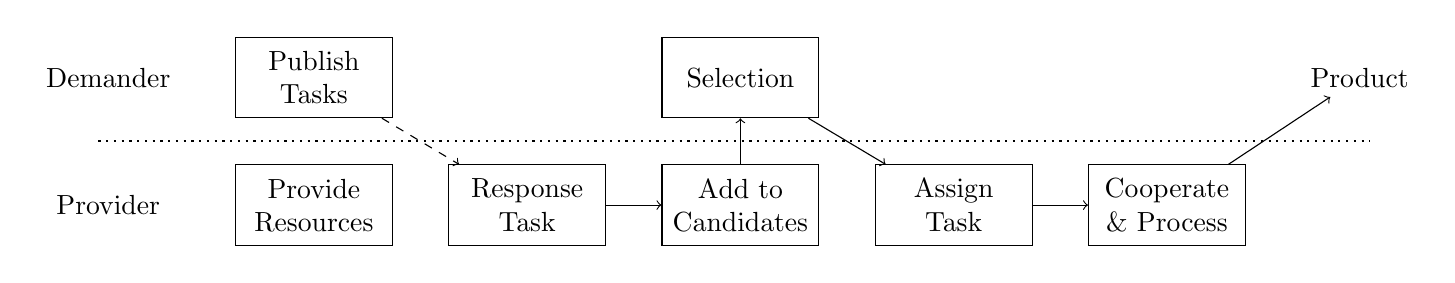
\begin{tikzpicture}[node distance=5mm and 5mm,
square/.style={
% The shape:
rectangle,
draw=black,
minimum size=2.9em,
text width=5em,
text centered
},
circle/.style={
rectangle,minimum size=1em,rounded corners=0.5em,
draw=black
}
]
\matrix[row sep=0.5em,column sep=2em] {
% First row:
\node (order) {Demander};& \node (task) [square]{Publish Tasks}; &  & \node (select) [square]{Selection}; & & &  \node (finish) {Product}; \\
\node (start) {}; & & & & & & \node (stop) {}; \\
\node (provider) {Provider};  & \node (resource) [square]{Provide Resources}; & \node (response) [square] {Response Task}; & \node (candidate) [square]{Add to Candidates}; & \node (match) [square]{Assign Task}; & \node (coord) [square] {Cooperate \& Process};&\\
};
\draw[dotted,thick] (start.west) -- (stop.east);
\path (task) edge[->,dashed] (response) (response) edge[->] (candidate) (candidate) edge[->] (select) (select) edge[->] (match) (match) edge[->] (coord) (coord) edge[->] (finish);
% \path (order) edge[->] (task) (task) edge[->] (match) (match) edge[->] (coord) (coord) edge[->] (process) (process) edge[->] (finish) (provider) edge[->] (resource) (resource) edge[->] (match);
\end{tikzpicture}